\subsubsection{UC\theuccount-G - GitLab segnala apertura issue al Producer GitLab}
	\begin{figure}[H]
		\centering
		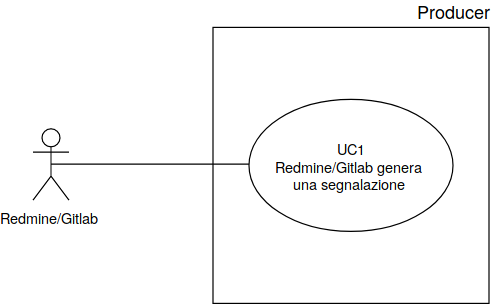
\includegraphics[width=0.7\textwidth]{img/UC1.png}\\
		\caption{UC\theuccount-G - GitLab segnala apertura issue al Producer GitLab}
	\end{figure}
	\begin{itemize}
		\item \textbf{Codice}: UC\theuccount-G.
		\item \textbf{Titolo}: GitLab segnala apertura issue al Producer GitLab.
		\item \textbf{Attori primari}: GitLab.
		\item \textbf{Descrizione}: l'invio di
		una segnalazione avviene da parte di GitLab tramite webhook. L'apertura di
		una issue su GitLab contiene:
		\begin{itemize}
			\item Title e opzionalmente:
			\begin{itemize}
				\item Label
				\item Milestone
				\item Assignees
				\item Due Date
			\end{itemize}
		\end{itemize}
		\item \textbf{Precondizione}: Viene aperta una issue su GitLab e 
		segnalata a \progetto.
		\item \textbf{Postcondizione}: il Producer GitLab riceve la segnalazione da GitLab.
		\item \textbf{Scenario principale}: 
		\begin{enumerate}
			\item GitLab procede all'invio della segnalazione di issue al Producer GitLab.
		\end{enumerate}
		
	\end{itemize}